\documentclass[11pt,a4paper]{article}

% ============================================================================
% PACKAGES
% ============================================================================
\usepackage[utf8]{inputenc}
\usepackage[T1]{fontenc}
\usepackage{amsmath,amssymb,amsthm}
\usepackage{mathtools}
\usepackage{algorithm}
\usepackage{algpseudocode}
\usepackage{graphicx}
\usepackage{booktabs}
\usepackage{multirow}
\usepackage{hyperref}
\usepackage{cleveref}
\usepackage{xcolor}
\usepackage{tikz}
\usetikzlibrary{shapes,arrows,positioning,fit,backgrounds,calc}
\usepackage[margin=1in]{geometry}
\usepackage{enumitem}
\usepackage{caption}
\usepackage{subcaption}

% ============================================================================
% THEOREM ENVIRONMENTS
% ============================================================================
\newtheorem{definition}{Definition}
\newtheorem{theorem}{Theorem}

% ============================================================================
% CUSTOM COMMANDS
% ============================================================================
\newcommand{\vect}[1]{\mathbf{#1}}
\newcommand{\mat}[1]{\mathbf{#1}}
\newcommand{\set}[1]{\mathcal{#1}}

% ============================================================================
% DOCUMENT
% ============================================================================
\begin{document}

\title{Methodology:\\Learning Automata for Adaptive Kelp Forest Monitoring}
\author{PhD Thesis Research \\ University of Victoria}
\date{\today}
\maketitle

\begin{abstract}
The goal of this chapter is to present a methodology for adaptive kelp forest monitoring that addresses a fundamental tension in satellite-based environmental monitoring: detection methods require feedback to improve, yet feedback arrives sparsely and unpredictably. In this work, we propose a Learning Automata framework that maintains a pool of diverse detection methods and learns to select among them based on environmental context. The framework comprises three integrated components, namely, global policy learning, context-aware adaptation, and sparse label handling. A central contribution of this work is the dual-layer non-stationarity model, a novel extension of classical Learning Automata theory that simultaneously handles changing environmental conditions and irregular feedback timing. We validate the approach using Leave-One-Site-Out evaluation across British Columbia's coastal kelp forests.
\end{abstract}

\tableofcontents
\newpage


% ============================================================================
\section{The Monitoring Challenge}
\label{sec:challenge}
% ============================================================================

British Columbia's kelp forests are among the most productive ecosystems on Earth. These underwater forests provide habitat for countless species, sequester carbon, and have sustained coastal First Nations communities for millennia. Today, they face unprecedented threats from climate change, marine heatwaves, and sea urchin predation. Monitoring these ecosystems at scale is essential for conservation. However, this monitoring task is surprisingly difficult.

Satellite remote sensing offers the spatial coverage needed for coastline-scale monitoring. Sensors such as Sentinel-2 capture imagery of BC's 25,000 kilometers of coastline every five days at 10-meter resolution. The challenge lies not in acquiring images, but in translating them into reliable kelp maps. Three interconnected problems make this translation fundamentally difficult.

\subsection{Environmental Heterogeneity}

No single detection algorithm works everywhere. A method optimized for calm summer waters fails when applied to turbid winter conditions. Bull kelp in exposed outer coastal environments behaves differently from bull kelp in protected inland waters. Kelp beds adjacent to sandy substrates exhibit different spectral characteristics than those over rocky reef. Further, river plumes, industrial activities, and adjacent land create site-specific detection challenges.

To render the problem concrete, consider a deep learning model trained on imagery from BC's central coast. Such a model learns the spectral signatures of kelp under those specific conditions, i.e., the water clarity, the substrate types, and the typical atmospheric conditions. When applied to the northern coast, with different water properties, different depths, and different adjacencies, performance degrades. The model has learned \emph{one} way to detect kelp, but kelp detection requires \emph{many} ways depending on context.

\subsection{Sparse and Delayed Validation}

Ground-truth validation data is expensive and logistically challenging to collect. Field surveys require boats, divers, and favorable weather. They cannot possibly keep pace with satellite image acquisition. A Sentinel-2 image captured today might not be validated for weeks or months, if it gets validated at all. Most images will never receive ground-truth labels.

This creates a fundamental tension. Detection methods require feedback to improve. However, feedback arrives irregularly and unpredictably. Traditional machine learning assumes dense, contemporaneous labels: one trains on labeled data, then deploys the model. In operational monitoring, however, the system must continue learning after deployment, using whatever sparse validation becomes available.

\subsection{Non-Stationary Conditions}

Both the environment and the observation process change over time. Seasonally, kelp forests undergo phenological cycles, namely, rapid growth in spring, peak canopy in summer, and senescence in fall. Water conditions vary with season as well: winter brings storms, turbidity, and low sun angles. The optimal detection strategy in August is not the optimal strategy in February.

On longer timescales, climate variability introduces regime shifts. El Ni\~{n}o events alter ocean temperatures and kelp physiology. Marine heatwaves can cause massive die-offs. A detection method tuned to ``normal'' conditions may fail during these anomalous periods.

The observation process is also non-stationary. Field validation follows seasonal patterns: most surveys happen in summer when conditions are favorable. Funding cycles, weather delays, and logistical constraints introduce year-to-year variability. Thus, the rate at which feedback arrives is itself unpredictable.

\subsection{The Core Question}

These challenges are interconnected. Environmental heterogeneity means different methods work in different contexts. Sparse feedback means we cannot simply train a new model for each context. Non-stationarity means even if we could, the optimal method would keep changing.

This raises the following question: \textbf{What if, instead of training a single ``best'' model, we maintained a pool of diverse detection methods and learned to select among them?} What if we could identify which method works best in which context, learn this mapping from sparse feedback, and adapt as conditions change?

This is precisely the approach we develop in this chapter.


% ============================================================================
\section{Key Insight: Selection Rather Than Training}
\label{sec:insight}
% ============================================================================

The conventional approach to machine learning treats model selection as a one-time decision. One trains several models, evaluates them on a validation set, selects the best one, and deploys it. The model is fixed; the world is assumed to be stationary.

We propose a fundamentally different approach: \textbf{treat model selection as an ongoing learning problem}. Rather than committing to a single detection method, we maintain a pool of diverse methods, each with different strengths and weaknesses, and learn to select among them based on environmental context.

\subsection{A Committee of Experts}

We can conceptualize this approach as a committee of experts, each trained under different conditions. One expert excels at detecting kelp in calm, clear water. Another handles turbid conditions well. A third is robust to low sun angles. When a new satellite image arrives, we examine the environmental context, i.e., water clarity, sun angle, season, and location, and select the expert most likely to succeed.

The selection is probabilistic, not deterministic. We maintain a probability distribution over the experts, representing our confidence in each one. If the committee has three experts, we might currently believe Expert A works well 60\% of the time, Expert B 30\%, and Expert C 10\%. When feedback arrives, i.e., a validated prediction, we update these probabilities. If Expert B performed better than expected, its probability increases; the others decrease.

Over time, the probability distribution converges. The system learns which experts to trust in which contexts. Moreover, this learning happens continuously, during deployment, from sparse feedback. We do not need to retrain models. We only require occasional validation to update our selection preferences.

\subsection{Why Learning Automata?}

This problem, i.e., selecting among actions based on probabilistic feedback, is precisely what Learning Automata (LA) are designed to solve. LA emerged from control theory in the 1960s as a framework for adaptive decision-making in unknown environments. An automaton maintains a probability distribution over actions, selects actions according to that distribution, receives rewards or penalties, and updates the distribution accordingly.

LA exhibit several properties that make them well-suited to our problem:

\begin{itemize}[noitemsep]
    \item \textbf{Sparse feedback tolerance:} LA do not require feedback on every action. They update only when feedback is available, and remain stable otherwise.

    \item \textbf{Non-stationarity handling:} LA can track changing environments. If the optimal action shifts over time, the probability distribution will eventually follow.

    \item \textbf{Convergence guarantees:} Under well-specified conditions, LA provably converge to the optimal action. This theoretical grounding distinguishes them from ad-hoc heuristics.

    \item \textbf{Simplicity:} The update rules are computationally lightweight. No gradient computation is required, no backpropagation; just probability adjustments.
\end{itemize}

We present the mathematics of LA in Appendix~\ref{app:la-theory}. For now, the intuition suffices. In summary, LA provide a principled way to learn which expert to trust, based on sparse feedback, in changing conditions.


% ============================================================================
\section{Framework Overview}
\label{sec:overview}
% ============================================================================

In this section, we describe the overall architecture of the adaptive monitoring framework. The system processes satellite imagery tiles and produces kelp detection maps, learning from sparse validation feedback to improve its selection decisions over time.

\subsection{System Architecture}

The framework comprises three integrated components, as illustrated in Figure~\ref{fig:architecture}:

\begin{figure}[h]
\centering
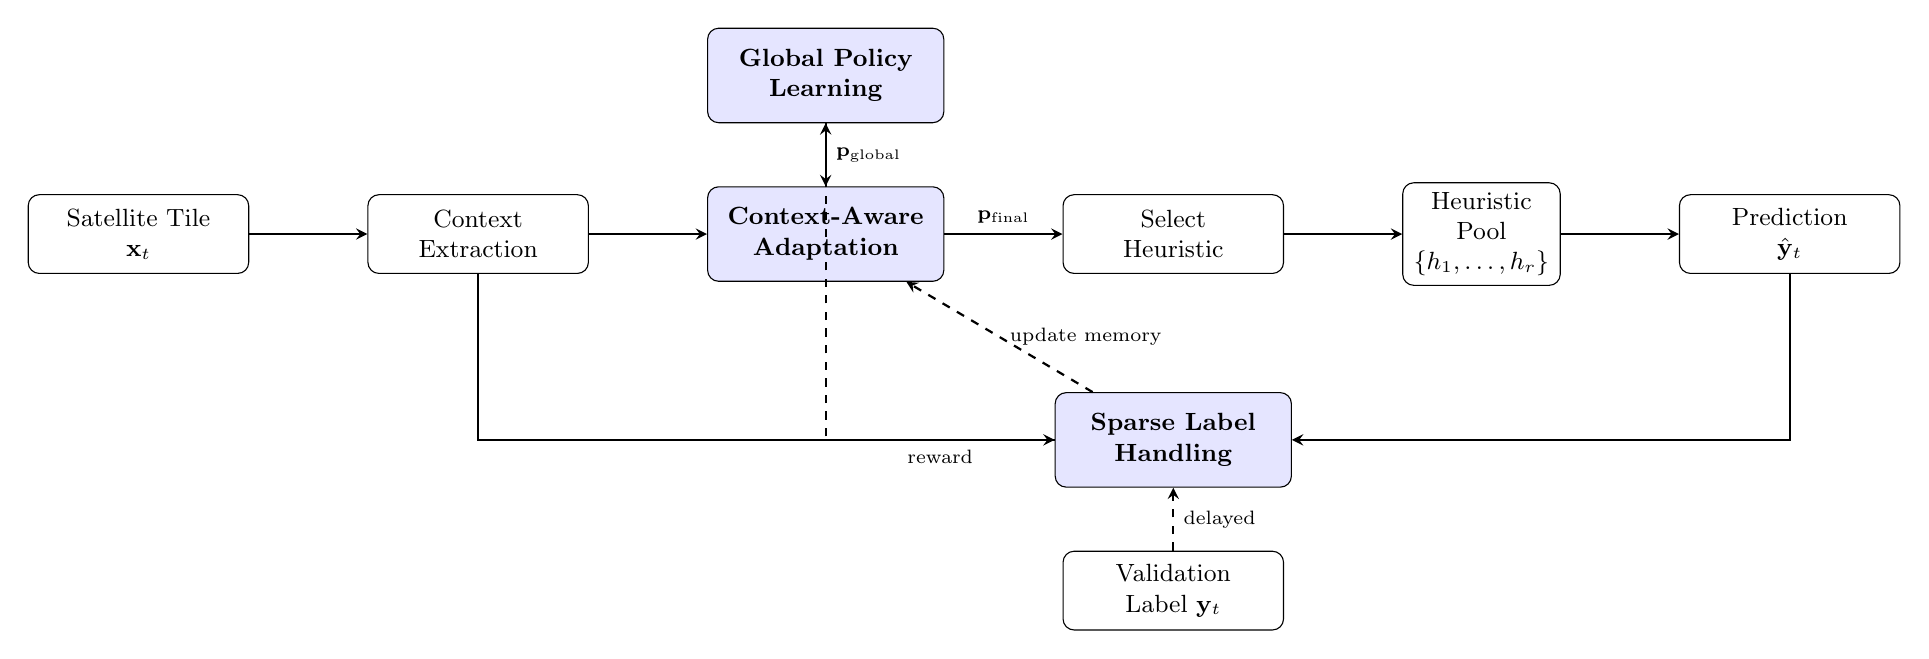
\begin{tikzpicture}[
    node distance=1.5cm,
    box/.style={rectangle, draw, rounded corners, minimum width=2.8cm, minimum height=1cm, align=center, font=\small},
    component/.style={rectangle, draw, rounded corners, fill=blue!10, minimum width=3cm, minimum height=1.2cm, align=center, font=\small\bfseries},
    arrow/.style={->, >=stealth, thick},
    dasharrow/.style={->, >=stealth, thick, dashed}
]
    % Input
    \node[box] (input) {Satellite Tile\\$\mathbf{x}_t$};

    % Context extraction
    \node[box, right=of input] (context) {Context\\Extraction};

    % Component 2
    \node[component, right=of context] (comp2) {Context-Aware\\Adaptation};

    % Component 1
    \node[component, above=0.8cm of comp2] (comp1) {Global Policy\\Learning};

    % Selection
    \node[box, right=of comp2] (select) {Select\\Heuristic};

    % Heuristic pool
    \node[box, right=of select, minimum width=2cm] (pool) {Heuristic\\Pool\\$\{h_1, \ldots, h_r\}$};

    % Prediction
    \node[box, right=of pool] (pred) {Prediction\\$\hat{\mathbf{y}}_t$};

    % Component 3
    \node[component, below=1.5cm of select] (comp3) {Sparse Label\\Handling};

    % Validation
    \node[box, below=0.8cm of comp3] (valid) {Validation\\Label $\mathbf{y}_t$};

    % Arrows
    \draw[arrow] (input) -- (context);
    \draw[arrow] (context) -- (comp2);
    \draw[arrow] (comp1) -- (comp2) node[midway, right, font=\scriptsize] {$\mathbf{p}_{\text{global}}$};
    \draw[arrow] (comp2) -- (select) node[midway, above, font=\scriptsize] {$\mathbf{p}_{\text{final}}$};
    \draw[arrow] (select) -- (pool);
    \draw[arrow] (pool) -- (pred);

    % To buffer
    \draw[arrow] (pred) |- (comp3);
    \draw[arrow] (context) |- (comp3);

    % From validation
    \draw[dasharrow] (valid) -- (comp3) node[midway, right, font=\scriptsize] {delayed};

    % Feedback loops
    \draw[dasharrow] (comp3) -| (comp1) node[near start, below, font=\scriptsize] {reward};
    \draw[dasharrow] (comp3) -- (comp2) node[midway, right, font=\scriptsize] {update memory};

\end{tikzpicture}
\caption{Framework architecture. Solid arrows show the inference path; dashed arrows show feedback paths that operate when validation labels arrive.}
\label{fig:architecture}
\end{figure}

\begin{enumerate}
    \item \textbf{Global Policy Learning} maintains a probability distribution over the pool of detection heuristics. This distribution encodes the system's overall preferences, i.e., which heuristics have performed well historically. When feedback arrives, the distribution updates according to Learning Automata rules.

    \item \textbf{Context-Aware Adaptation} extracts environmental features from each input tile and uses a memory bank of past experiences to adapt the global preferences to the current context. In familiar conditions, it trusts past experience; in novel conditions, it falls back to global preferences.

    \item \textbf{Sparse Label Handling} buffers predictions awaiting validation. When ground-truth labels eventually arrive, perhaps days, weeks, or months later, it retrieves the corresponding predictions, computes rewards, and triggers updates to Components 1 and 2.
\end{enumerate}

\subsection{The Inference Path}

When a new satellite tile arrives, the system processes it as follows:

\begin{enumerate}
    \item \textbf{Extract context.} We compute environmental features from the tile, namely, spectral statistics, texture measures, temporal metadata (day of year), and geographic location. These features form a context vector describing the current conditions.

    \item \textbf{Blend global and local preferences.} Using the context vector, we query the memory bank for similar past conditions. If similar contexts exist with consistent performance records, we blend their preferences with the global policy. If the context is novel, we rely primarily on the global policy.

    \item \textbf{Select a heuristic.} We sample a detection heuristic according to the blended probability distribution. The selection is stochastic; even low-probability heuristics occasionally get selected, enabling continued exploration.

    \item \textbf{Generate prediction.} The selected heuristic processes the tile and produces a binary kelp/no-kelp mask.

    \item \textbf{Buffer the prediction.} The prediction, along with the context vector and selected heuristic index, enters a buffer awaiting validation.
\end{enumerate}

\subsection{The Feedback Path}

When a validation label arrives, perhaps weeks after the original prediction, we process it as follows:

\begin{enumerate}
    \item \textbf{Retrieve the buffered prediction.} Using location and timestamp, we look up the corresponding entry in the buffer.

    \item \textbf{Compute the reward.} We measure how well the prediction matched the ground truth, typically using Intersection over Union (IoU).

    \item \textbf{Update the global policy.} The reward signal adjusts the probability distribution over heuristics. Good performance increases the selected heuristic's probability; poor performance decreases it (or leaves it unchanged, depending on the LA scheme).

    \item \textbf{Update the memory bank.} We store the context vector and observed performance, enriching future context-aware adaptation.
\end{enumerate}

Thus, the key insight is that these feedback updates are \emph{decoupled} from inference. The system continues making predictions without waiting for validation. When validation arrives, the system learns. However, learning is asynchronous, sparse, and delayed.


% ============================================================================
\section{Component 1: Learning What Works}
\label{sec:component1}
% ============================================================================

The first component maintains the system's global preferences over detection heuristics. We can conceptualize this as the system's ``overall opinion'' about which methods tend to work well, averaged across all contexts it has encountered.

\subsection{The Probability Distribution}

The global policy is a probability distribution over $r$ heuristics:
\[
\mathbf{p} = [p_1, p_2, \ldots, p_r]
\]
where each $p_i$ represents the system's confidence in heuristic $h_i$. Initially, the distribution is uniform; the system has no prior preference:
\[
p_i(0) = \frac{1}{r} \quad \text{for all } i
\]

As feedback accumulates, the distribution evolves. Heuristics that consistently perform well accumulate probability mass; those that underperform lose it. Eventually, the distribution concentrates on the best-performing heuristics.

\subsection{The Update Rule}

When validation arrives for a prediction made using heuristic $h_i$, we compute a reward based on detection accuracy. The reward $R$ ranges from 0 (complete failure) to 1 (perfect detection).

The probability update depends on the Learning Automata scheme. The simplest scheme, Linear Reward-Inaction (L$_{\text{R-I}}$), updates only on positive feedback:

\begin{itemize}
    \item If the reward exceeds a threshold (good performance), increase $p_i$ and decrease the others proportionally.
    \item If the reward is below the threshold (poor performance), do nothing.
\end{itemize}

This ``inaction on penalty'' makes the system robust to noise. A single poor performance does not immediately punish a heuristic; only consistent good performance is rewarded. We provide the formal update equations in Appendix~\ref{app:la-theory}.

Other schemes, namely, Linear Reward-Penalty, Pursuit, and Variable Structure, offer different tradeoffs between learning speed and stability. We experiment with six variants, described in Appendix~\ref{app:la-theory}, and identify which work best for kelp detection through ablation studies.

\subsection{Why This Works}

The global policy serves as the system's ``default'' preference. Without context-specific information, it represents the best available guess. Its strength lies in aggregating experience across all contexts: if heuristic $h_3$ performs well 70\% of the time across diverse conditions, this gets reflected in a high $p_3$.

However, global preferences are blunt instruments. A heuristic that excels in summer may struggle in winter. The global policy averages over these variations. Thus, to exploit context-specific patterns, we require the second component.


% ============================================================================
\section{Component 2: Adapting to Context}
\label{sec:component2}
% ============================================================================

The second component enables the system to adapt its heuristic selection based on environmental context. The intuition is straightforward: when current conditions resemble past conditions where a particular heuristic excelled, we favor that heuristic.

\subsection{Context Features}

Each satellite tile carries information about the environmental conditions under which it was captured. We extract a context vector $\mathbf{c}$ encoding:

\begin{itemize}[noitemsep]
    \item \textbf{Spectral statistics:} Mean and variance of each spectral band, capturing water color, turbidity, and atmospheric conditions.
    \item \textbf{Spatial texture:} Entropy and homogeneity measures, indicating surface roughness and wave state.
    \item \textbf{Temporal context:} Day of year, capturing seasonal patterns.
    \item \textbf{Geographic location:} Latitude and longitude, capturing regional characteristics.
    \item \textbf{Auxiliary data:} Bathymetry and substrate type, when available.
\end{itemize}

This context vector summarizes the type of conditions we are dealing with. Two tiles with similar context vectors likely require similar detection strategies.

\subsection{The Memory Bank}

We maintain a memory bank of past experiences:
\[
\mathcal{M} = \{(\mathbf{c}_j, \mathbf{p}_j, R_j)\}
\]
Each entry records a context vector, the heuristic selection probabilities used in that context, and the reward obtained. Over time, the memory bank accumulates a record of what worked where.

When a new tile arrives with context $\mathbf{c}$, we retrieve the $k$ most similar past contexts using nearest-neighbor search. For efficiency with large memory banks, we employ FAISS, a library for fast approximate nearest-neighbor search.

\subsection{Local Preference Estimation}

The retrieved neighbors provide evidence about what works in similar conditions. We compute a local preference distribution by averaging the neighbors' preferences, weighted by their rewards and similarity.

The neighbors that (a) are more similar to the current context and (b) achieved higher rewards contribute more to the local estimate. The result of such a process is a distribution $\mathbf{p}_{\text{local}}$ that reflects ``what has worked in conditions like these.''

\subsection{Blending Global and Local}

The final selection probability blends global and local preferences:
\begin{equation}
\mathbf{p}_{\text{final}} = \alpha \cdot \mathbf{p}_{\text{global}} + (1 - \alpha) \cdot \mathbf{p}_{\text{local}}
\label{eq:blending}
\end{equation}

The blending coefficient $\alpha$ controls the balance:
\begin{itemize}
    \item When $\alpha = 1$: Trust only the global policy (ignore local context).
    \item When $\alpha = 0$: Trust only local experience (ignore global trends).
    \item In between: Blend both sources of information.
\end{itemize}

We make $\alpha$ adaptive. When the memory bank contains many similar contexts with consistent outcomes, $\alpha$ decreases; we trust local experience. When contexts are novel or outcomes inconsistent, $\alpha$ increases; we fall back to global preferences.

\subsection{Why This Works}

Context-aware adaptation exploits structure in the problem. Environmental conditions are not random; they cluster. Turbid winter conditions in the Strait of Georgia are similar to other turbid winter conditions in the same region. Thus, if a particular heuristic succeeds in those conditions, it likely will again.

The memory bank provides non-parametric generalization. We do not train a model to predict heuristic performance from context features. We simply remember what worked and retrieve it when relevant. This approach is robust, interpretable, and requires no additional training.


% ============================================================================
\section{Component 3: Learning from Sparse Feedback}
\label{sec:component3}
% ============================================================================

The third component handles the operational reality that validation labels arrive sparsely and with variable delay. Most predictions will never be validated. Those that are may be validated days, weeks, or months after the fact. The system must continue operating without waiting for feedback, yet learn when feedback becomes available.

\subsection{The Prediction Buffer}

Every prediction enters a buffer:
\[
\mathcal{B} = \{(t_j, \mathbf{c}_j, i_j, \hat{\mathbf{y}}_j)\}
\]
Each entry records the timestamp, context vector, selected heuristic index, and predicted mask. A hash map enables efficient lookup by location and time.

When a validation label arrives for a particular location and date, we retrieve the corresponding buffered prediction, compute the reward, and trigger updates to Components 1 and 2. We then remove the entry from the buffer.

\subsection{Buffer Management}

Predictions cannot wait indefinitely. Environmental conditions change; a prediction made six months ago may no longer be relevant to current learning. We impose a maximum buffer age (e.g., 6 months). Predictions older than this threshold are discarded without update.

This reflects our design philosophy: \textbf{the system should learn from timely feedback, not stale feedback}. A reward received promptly is more informative than one received after conditions have shifted.

\subsection{Temporal Decay}

Optionally, rewards can be discounted based on delay:
\begin{equation}
R_{\text{effective}} = R \cdot \gamma^{\delta}
\label{eq:decay}
\end{equation}
where $\delta$ is the delay (in days) between prediction and validation, and $\gamma < 1$ is a decay factor. Recent feedback receives full weight; older feedback is down-weighted.

This decay serves two purposes:
\begin{enumerate}
    \item \textbf{Prioritizing recency:} Recent experience is more relevant to current conditions.
    \item \textbf{Tracking non-stationarity:} If the optimal heuristic changes over time, discounting old rewards helps the system adapt.
\end{enumerate}

\subsection{Learning Without Waiting}

The critical design principle is \textbf{asynchronous learning}. The inference path, i.e., tile in, prediction out, operates continuously without blocking on validation. The feedback path, i.e., label in, update out, operates whenever labels arrive. These two paths are decoupled.

This design matches the operational reality of environmental monitoring. Satellites capture imagery every few days. Field validation happens when resources and conditions permit. The system cannot wait for validation before making predictions. However, it can learn from validation whenever it arrives.


% ============================================================================
\section{Novel Contribution: Dual-Layer Non-Stationarity}
\label{sec:dual-layer}
% ============================================================================

Classical Learning Automata theory addresses non-stationary environments where the optimal action changes over time. In this work, we extend this theory to model a \textbf{second layer of non-stationarity}: not just \emph{what} is optimal, but \emph{when we learn about it}.

\subsection{Two Sources of Change}

Kelp forest monitoring exhibits two distinct sources of non-stationarity that must be handled simultaneously:

\begin{figure}[h]
\centering
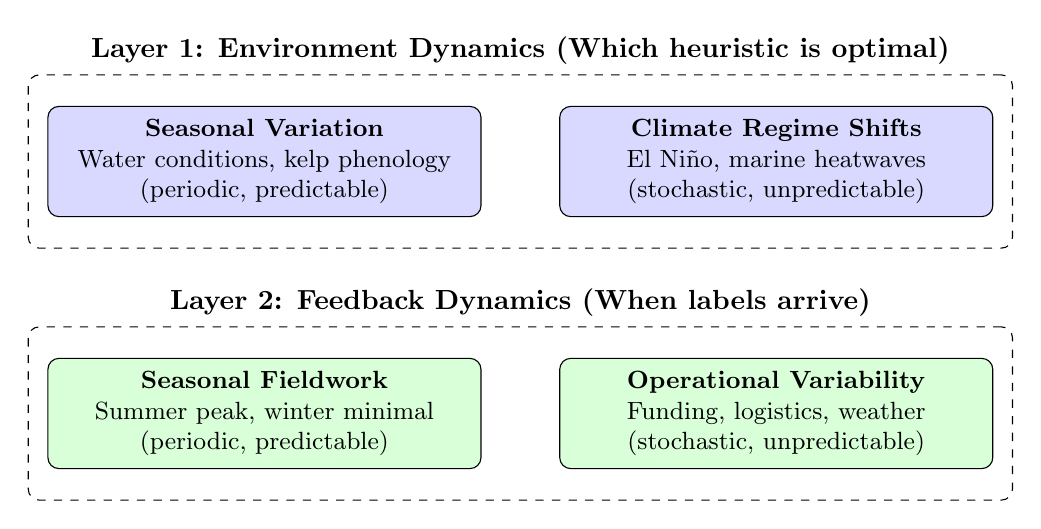
\begin{tikzpicture}[
    box/.style={rectangle, draw, rounded corners, minimum width=5.5cm, minimum height=1.4cm, align=center, font=\small},
    layer/.style={rectangle, draw, dashed, rounded corners, minimum width=12.5cm, minimum height=2.2cm}
]
    % Layer 1
    \node[box, fill=blue!15] (layer1-pse) at (-3, 2) {\textbf{Seasonal Variation}\\Water conditions, kelp phenology\\(periodic, predictable)};
    \node[box, fill=blue!15] (layer1-mse) at (3.5, 2) {\textbf{Climate Regime Shifts}\\El Ni\~{n}o, marine heatwaves\\(stochastic, unpredictable)};
    \node[layer, fit=(layer1-pse)(layer1-mse), label={[font=\bfseries]above:Layer 1: Environment Dynamics (Which heuristic is optimal)}] {};

    % Layer 2
    \node[box, fill=green!15] (layer2-pse) at (-3, -1.2) {\textbf{Seasonal Fieldwork}\\Summer peak, winter minimal\\(periodic, predictable)};
    \node[box, fill=green!15] (layer2-mse) at (3.5, -1.2) {\textbf{Operational Variability}\\Funding, logistics, weather\\(stochastic, unpredictable)};
    \node[layer, fit=(layer2-pse)(layer2-mse), label={[font=\bfseries]above:Layer 2: Feedback Dynamics (When labels arrive)}] {};
\end{tikzpicture}
\caption{Dual-layer non-stationarity model. Layer 1 governs which detection method is optimal. Layer 2 governs when validation feedback is available. Both layers combine periodic (seasonal) and stochastic (inter-annual) components.}
\label{fig:dual-layer}
\end{figure}

\subsubsection{Layer 1: Environment Dynamics}

This layer models how the \textbf{optimal detection heuristic} changes over time. Two mechanisms drive this change:

\begin{itemize}
    \item \textbf{Seasonal variation (periodic):} Kelp forests undergo annual cycles. In summer, canopies are fully developed and easily detectable. In winter, storms reduce canopy extent and turbidity obscures detection. A heuristic optimized for calm summer water may fail in turbid winter conditions. Thus, the optimal heuristic follows a predictable seasonal pattern.

    \item \textbf{Climate regime shifts (stochastic):} Interannual variability introduces unpredictable shifts. El Ni\~{n}o events alter water temperatures and kelp physiology. Marine heatwaves cause unprecedented conditions. These shifts change which heuristic performs best, but they do not follow a predictable schedule.
\end{itemize}

In classical LA theory, these are called Periodic Switching Environments (PSE) and Markovian Switching Environments (MSE), respectively. Layer 1 combines both.

\subsubsection{Layer 2: Feedback Dynamics}

This layer models \textbf{when validation labels arrive}. This is our novel extension to LA theory. Two mechanisms drive feedback timing:

\begin{itemize}
    \item \textbf{Seasonal fieldwork (periodic):} Most validation surveys happen in summer, when weather and sea conditions favor boat-based fieldwork. Winter validation is rare. Thus, the probability of receiving feedback follows a seasonal pattern.

    \item \textbf{Operational variability (stochastic):} Research funding fluctuates. Field crews have varying availability. Weather delays and equipment failures introduce unpredictable gaps. Some years produce abundant validation data; others produce little.
\end{itemize}

Layer 2 is \textbf{independent} of Layer 1. A summer day might have both optimal detection conditions (Layer 1) and high feedback probability (Layer 2). A winter day might have challenging detection conditions (Layer 1) and low feedback probability (Layer 2). The two layers do not necessarily align.

\subsection{Why This Matters}

Classical LA theory focuses on Layer 1: the environment changes, and the automaton must track the changing optimal action. However, this theory implicitly assumes that feedback arrives regularly. In practice, feedback arrives according to its own dynamics.

The dual-layer model captures this reality:
\begin{itemize}
    \item \textbf{The system faces periods of feedback drought.} In winter, months may pass without validation. The system must maintain stable behavior without updates.

    \item \textbf{The system faces feedback bursts.} In summer, multiple surveys may validate predictions rapidly. The system must incorporate this feedback efficiently.

    \item \textbf{The optimal action and feedback availability may be anti-correlated.} Winter conditions (where certain heuristics excel) produce little validation. The system may learn less about precisely those conditions where adaptation is most needed.
\end{itemize}

By modeling both layers explicitly, we can analyze learning dynamics under realistic conditions. We can design LA schemes that remain stable during droughts and responsive during bursts. We can test robustness to different feedback patterns.

\subsection{Scientific Contribution}

The dual-layer non-stationarity model makes three contributions:

\begin{enumerate}
    \item \textbf{Novel theoretical extension:} We extend classical LA theory on non-stationary environments to include feedback timing as a separate stochastic process. This opens new analytical questions: How does learning degrade under sparse feedback? What LA schemes are most robust to feedback timing variability?

    \item \textbf{Domain-appropriate modeling:} The formulation captures genuine characteristics of environmental monitoring. Seasonal patterns and operational variability are real. Modeling them explicitly improves realism.

    \item \textbf{Ablation capability:} The two layers are independently configurable. We can test Layer 1 effects (environment dynamics) while holding Layer 2 constant, and vice versa. This enables rigorous experimental analysis of how each source of non-stationarity affects learning.
\end{enumerate}


% ============================================================================
\section{Evaluation Strategy}
\label{sec:evaluation}
% ============================================================================

We evaluate the framework on kelp forest imagery from British Columbia's coast, using Leave-One-Site-Out cross-validation and a staged ablation protocol.

\subsection{Datasets}

\begin{table}[h]
\centering
\caption{Datasets used for evaluation}
\label{tab:datasets}
\begin{tabular}{lccp{5cm}}
\toprule
\textbf{Dataset} & \textbf{Images} & \textbf{Labels} & \textbf{Purpose} \\
\midrule
BC Sentinel-2 (Labeled) & 7 & Yes & Primary training and validation \\
BC Sentinel-2 (Multi-temporal) & $\sim$100 & No & Layer 1 testing, sparse simulation \\
Figshare Landsat & 432 & Yes & Cross-sensor transfer \\
\bottomrule
\end{tabular}
\end{table}

The primary dataset consists of Sentinel-2 imagery from seven sites along BC's coast, with expert-labeled kelp masks. Each tile is 512$\times$512 pixels at 10-meter resolution, containing 12 spectral and auxiliary bands. We provide full dataset specifications in Appendix~\ref{app:datasets}.

\subsection{Heuristic Pool}

The heuristic pool comprises:
\begin{itemize}[noitemsep]
    \item \textbf{Ten site-specific models:} UNet-MaxViT architectures trained using Leave-One-Site-Out protocol. Each model has seen different training conditions.
    \item \textbf{One RGB model:} Trained on all BC sites using only visual bands, enabling cross-sensor transfer to Landsat imagery.
\end{itemize}

\subsection{Leave-One-Site-Out Protocol}

For primary evaluation, we hold out one site at a time:
\begin{enumerate}
    \item Train the LA framework on six sites.
    \item Evaluate on the held-out seventh site.
    \item Repeat for all seven sites.
    \item Aggregate results.
\end{enumerate}

This protocol tests generalization to unseen geographic regions, a critical capability for coastline-scale deployment.

\subsection{Staged Ablation}

Full factorial evaluation of all design choices would require tens of thousands of experiments. To render the experimental design practical, we employ a staged approach:

\begin{enumerate}
    \item \textbf{Stage 1: LA variant selection.} We compare six LA schemes (L$_{\text{R-I}}$, L$_{\text{R-P}}$, VSLA, Pursuit, Discretized Pursuit, SERI) with the full system. We identify the top 2--3 performers.

    \item \textbf{Stage 2: Component ablation.} We test combinations of components (global only, global+context, global+sparse, full system) with top LA variants.

    \item \textbf{Stage 3: Sparsity tolerance.} We vary label density (100\%, 50\%, 10\%, 5\%) and delay patterns with the best configuration.

    \item \textbf{Stage 4: Auxiliary data.} We test with/without bathymetry, substrate, and other auxiliary layers.

    \item \textbf{Stage 5: Cross-sensor transfer.} We evaluate on Figshare Landsat using the RGB model.
\end{enumerate}

This staged approach reduces computational requirements from $>$46,000 runs to $\sim$500 while maintaining scientific rigor.

\subsection{Baselines}

We compare against:
\begin{itemize}[noitemsep]
    \item \textbf{Random selection:} Uniform random choice among heuristics.
    \item \textbf{Best single heuristic:} The fixed heuristic that performs best overall.
    \item \textbf{Oracle:} The best heuristic for each tile (upper bound requiring perfect foresight).
\end{itemize}

\subsection{Metrics}

Primary detection metrics:
\begin{itemize}[noitemsep]
    \item \textbf{Intersection over Union (IoU):} Overlap between predicted and true kelp masks.
    \item \textbf{F1-score:} Harmonic mean of precision and recall.
\end{itemize}

LA-specific metrics:
\begin{itemize}[noitemsep]
    \item \textbf{Convergence speed:} Steps to reach 90\% of final performance.
    \item \textbf{Final entropy:} Concentration of the probability distribution at convergence.
\end{itemize}

We provide formal definitions in Appendix~\ref{app:metrics}.


% ============================================================================
\section{Summary}
\label{sec:summary}
% ============================================================================

In this chapter, we presented a methodology for adaptive kelp forest monitoring that addresses fundamental challenges in satellite-based environmental observation.

\textbf{The core insight} is to treat detection as a selection problem rather than a training problem. Thus, instead of building one model that must work everywhere, we maintain a pool of diverse methods and learn to select among them based on context.

\textbf{The framework} comprises three components:
\begin{enumerate}
    \item Global policy learning, which tracks overall heuristic performance using Learning Automata.
    \item Context-aware adaptation, which tailors selection to environmental conditions using memory-based retrieval.
    \item Sparse label handling, which enables learning from irregular, delayed validation feedback.
\end{enumerate}

\textbf{The novel contribution} is the dual-layer non-stationarity model, which extends classical LA theory to handle both changing environmental conditions (Layer 1) and irregular feedback timing (Layer 2). This provides theoretical grounding for learning under the realistic constraints of operational monitoring.

\textbf{Evaluation} uses Leave-One-Site-Out cross-validation across BC's coastal kelp forests, with staged ablations to identify effective configurations and test robustness to sparse feedback.

The following chapters present experimental results validating each component and demonstrating the framework's effectiveness for adaptive kelp forest monitoring.


% ============================================================================
% APPENDICES
% ============================================================================
\appendix

\section{Formal Problem Definition}
\label{app:formal}

\subsection{Input Space}

Let $\mathbf{x}_t \in \mathbb{R}^{B \times H \times W}$ denote a satellite image tile acquired at time $t$, where $B$ is the number of spectral bands and $H \times W$ the spatial dimensions. For Sentinel-2: $B = 12$, $H = W = 512$, at 10m resolution.

The context vector $\mathbf{c}_t \in \mathbb{R}^D$ encodes environmental conditions:
\begin{equation}
\mathbf{c}_t = \left[ \mathbf{c}^{\text{spectral}}_t, \mathbf{c}^{\text{spatial}}_t, \mathbf{c}^{\text{temporal}}_t, \mathbf{c}^{\text{environ}}_t, \mathbf{c}^{\text{geo}}_t \right]^\top
\end{equation}

\subsection{Heuristic Pool}

The heuristic pool $\mathcal{H} = \{h_1, \ldots, h_r\}$ contains $r$ detection methods, each mapping tiles to binary masks:
\begin{equation}
h_i : \mathbb{R}^{B \times H \times W} \rightarrow \{0, 1\}^{H \times W}
\end{equation}

\subsection{Reward Function}

The primary reward is Intersection over Union:
\begin{equation}
R(\hat{\mathbf{y}}, \mathbf{y}) = \text{IoU}(\hat{\mathbf{y}}, \mathbf{y}) = \frac{|\hat{\mathbf{y}} \cap \mathbf{y}|}{|\hat{\mathbf{y}} \cup \mathbf{y}|} = \frac{\text{TP}}{\text{TP} + \text{FP} + \text{FN}}
\end{equation}

\subsection{Policy Objective}

We learn a policy $\pi : (\mathbf{x}, \mathbf{c}) \rightarrow \Delta^{r-1}$ maximizing expected reward:
\begin{equation}
\pi^* = \arg\max_\pi \mathbb{E}_{(\mathbf{x}, \mathbf{c}, \mathbf{y}) \sim \mathcal{D}} \left[ \sum_{i=1}^{r} \pi(\mathbf{x}, \mathbf{c})_i \cdot R(h_i(\mathbf{x}), \mathbf{y}) \right]
\end{equation}


\section{Learning Automata Theory}
\label{app:la-theory}

\subsection{Basic Formulation}

\begin{definition}[Learning Automaton]
A Learning Automaton is defined by $\langle \mathcal{A}, \mathcal{R}, \mathbf{p}, T \rangle$ where:
\begin{itemize}[noitemsep]
    \item $\mathcal{A} = \{\alpha_1, \ldots, \alpha_r\}$: action set
    \item $\mathcal{R} = \{0, 1\}$: response set (penalty, reward)
    \item $\mathbf{p}(n) = [p_1(n), \ldots, p_r(n)]^\top$: action probability vector at step $n$
    \item $T$: probability update rule
\end{itemize}
\end{definition}

The environment has penalty probabilities $\{c_1, \ldots, c_r\}$ where $c_i = P(\beta = 0 \mid \alpha = \alpha_i)$.

\subsection{Linear Reward-Inaction (L$_{\text{R-I}}$)}

Update on reward only:
\begin{align}
\text{If } \beta(n) = 1: \quad & p_i(n+1) = p_i(n) + \alpha(1 - p_i(n)) \quad \text{(selected action)} \\
& p_j(n+1) = p_j(n)(1 - \alpha) \quad j \neq i \\
\text{If } \beta(n) = 0: \quad & p_i(n+1) = p_i(n) \quad \forall i
\end{align}

\begin{theorem}[L$_{\text{R-I}}$ Convergence]
For distinct penalty probabilities $c_1 < c_2 < \cdots < c_r$, L$_{\text{R-I}}$ converges almost surely to the optimal action.
\end{theorem}

\subsection{Linear Reward-Penalty (L$_{\text{R-P}}$)}

Update on both reward and penalty:
\begin{align}
\text{If } \beta(n) = 1: \quad & p_i(n+1) = p_i(n) + \alpha(1 - p_i(n)) \\
& p_j(n+1) = p_j(n)(1 - \alpha) \quad j \neq i \\
\text{If } \beta(n) = 0: \quad & p_i(n+1) = p_i(n)(1 - \beta) \\
& p_j(n+1) = p_j(n) + \frac{\beta}{r-1}(1 - p_j(n)) \quad j \neq i
\end{align}

\subsection{Pursuit Automata}

We maintain reward estimates $\hat{d}_i(n)$ and pursue the current best:
\begin{align}
\hat{d}_i(n) &= \frac{\text{Total rewards for } \alpha_i}{\text{Total selections of } \alpha_i} \\
m(n) &= \arg\max_i \hat{d}_i(n) \\
p_{m(n)}(n+1) &= p_{m(n)}(n) + \alpha(1 - p_{m(n)}(n))
\end{align}

\subsection{Variable Structure LA (VSLA)}

Adaptive learning rate based on entropy:
\begin{align}
H(\mathbf{p}) &= -\sum_{i=1}^{r} p_i \log_2 p_i \\
\alpha(n) &= \alpha_{\min} + (\alpha_{\max} - \alpha_{\min}) \cdot \frac{H(\mathbf{p}(n))}{\log_2 r}
\end{align}

\subsection{Stochastic Estimator Reward-Inaction (SERI)}

Bayesian estimation with Beta posteriors:
\begin{equation}
p(\theta_i \mid \text{data}) \propto \text{Beta}(\alpha_i, \beta_i)
\end{equation}
Combined with pursuit-style updates. This is among the fastest $\epsilon$-optimal algorithms.


\section{Algorithm Pseudocode}
\label{app:algorithms}

\begin{algorithm}[H]
\caption{Framework Inference}
\begin{algorithmic}[1]
\Require Tile $\mathbf{x}$, global policy $\mathbf{p}_{\text{global}}$, memory bank $\mathcal{M}$
\State $\mathbf{c} \gets \text{ExtractContext}(\mathbf{x})$
\State $\mathcal{N}_k \gets \text{kNN}(\mathbf{c}, \mathcal{M}, k)$
\State $\mathbf{p}_{\text{local}} \gets \text{WeightedAverage}(\mathcal{N}_k)$
\State $\alpha \gets \text{ComputeBlendingCoef}(\mathcal{N}_k)$
\State $\mathbf{p}_{\text{final}} \gets \alpha \cdot \mathbf{p}_{\text{global}} + (1-\alpha) \cdot \mathbf{p}_{\text{local}}$
\State $i \sim \text{Categorical}(\mathbf{p}_{\text{final}})$
\State $\hat{\mathbf{y}} \gets h_i(\mathbf{x})$
\State $\mathcal{B} \gets \mathcal{B} \cup \{(t, \mathbf{c}, i, \hat{\mathbf{y}})\}$ \Comment{Buffer prediction}
\State \Return $\hat{\mathbf{y}}$
\end{algorithmic}
\end{algorithm}

\begin{algorithm}[H]
\caption{Label Arrival Processing}
\begin{algorithmic}[1]
\Require Validation label $\mathbf{y}$ for location $\ell$, time $t$
\State $(t_j, \mathbf{c}_j, i_j, \hat{\mathbf{y}}_j) \gets \mathcal{B}[\text{lookup}(\ell, t)]$
\State $\delta \gets t_{\text{current}} - t_j$ \Comment{Delay}
\If{$\delta > T_{\max}$}
    \State Remove from buffer; \Return \Comment{Too old}
\EndIf
\State $R \gets \text{IoU}(\hat{\mathbf{y}}_j, \mathbf{y}) \cdot \gamma^\delta$ \Comment{Reward with decay}
\State $\mathbf{p}_{\text{global}} \gets \text{LAUpdate}(\mathbf{p}_{\text{global}}, i_j, R)$ \Comment{Update Component 1}
\State $\mathcal{M} \gets \mathcal{M} \cup \{(\mathbf{c}_j, \mathbf{p}_{\text{final}}, R)\}$ \Comment{Update Component 2}
\State Remove entry from $\mathcal{B}$
\end{algorithmic}
\end{algorithm}


\section{Dataset Details}
\label{app:datasets}

\subsection{BC Sentinel-2 Dataset}

\begin{table}[h]
\centering
\caption{BC Sentinel-2 sites}
\begin{tabular}{llllc}
\toprule
\textbf{Site} & \textbf{UTM} & \textbf{Date} & \textbf{Season} & \textbf{Tiles} \\
\midrule
T09UXQ & 9U & July 27, 2021 & Summer & $\sim$40 \\
T09UYQ & 9U & August 6, 2022 & Summer & $\sim$45 \\
T10UCU & 10U & August 6, 2022 & Summer & $\sim$50 \\
T09UXS & 9U & August 4, 2023 & Summer & $\sim$35 \\
T10UCA & 10U & August 16, 2023 & Summer & $\sim$40 \\
T09UWT & 9U & August 19, 2023 & Summer & $\sim$45 \\
T09UUU & 9U & September 2, 2023 & Summer & $\sim$42 \\
\midrule
\multicolumn{4}{l}{\textbf{Total}} & $\sim$300 \\
\bottomrule
\end{tabular}
\end{table}

\subsection{Band Specification}

\begin{table}[h]
\centering
\caption{12-band tile structure}
\begin{tabular}{cll}
\toprule
\textbf{Band} & \textbf{Source} & \textbf{Resolution} \\
\midrule
1--4 & B2, B3, B4, B8 & 10m (native) \\
5--10 & B5, B6, B7, B8A, B11, B12 & 10m (resampled from 20m) \\
11 & Substrate classification & 10m (resampled) \\
12 & Bathymetry & 10m (resampled) \\
\bottomrule
\end{tabular}
\end{table}


\section{Metrics Definitions}
\label{app:metrics}

\subsection{Detection Metrics}

\begin{align}
\text{IoU} &= \frac{\text{TP}}{\text{TP} + \text{FP} + \text{FN}} \\
\text{Precision} &= \frac{\text{TP}}{\text{TP} + \text{FP}} \\
\text{Recall} &= \frac{\text{TP}}{\text{TP} + \text{FN}} \\
\text{F1} &= 2 \cdot \frac{\text{Precision} \cdot \text{Recall}}{\text{Precision} + \text{Recall}}
\end{align}

\subsection{LA Metrics}

\begin{align}
\text{Entropy} &= H(\mathbf{p}) = -\sum_{i=1}^{r} p_i \log_2 p_i \\
\text{Convergence} &= \min\{n : \text{IoU}(n) \geq 0.9 \cdot \text{IoU}_{\text{final}}\}
\end{align}


% ============================================================================
% BIBLIOGRAPHY
% ============================================================================
\bibliographystyle{plain}
\begin{thebibliography}{99}

\bibitem{narendra1989}
K.~S. Narendra and K.~S. Thathachar.
\newblock {\em Learning Automata: An Introduction}.
\newblock Prentice Hall, 1989.

\bibitem{thathachar2002}
M.~A.~L. Thathachar and P.~S. Sastry.
\newblock Varieties of learning automata: An overview.
\newblock {\em IEEE Trans. Systems, Man, and Cyberntic, Part B}, 32(6):711--722, 2002.

\bibitem{schroeder2020}
S.~B. Schroeder, C.~Dupont, L.~Boyer, F.~Juanes, and M.~Costa.
\newblock Passive remote sensing technology for mapping bull kelp.
\newblock {\em Global Ecology and Conservation}, 22:e00948, 2020.

\bibitem{starko2024}
S.~Starko et~al.
\newblock Heterogeneity in BC kelp forest communities.
\newblock {\em Journal of Phycology}, 2024.

\bibitem{mora-soto2024}
A.~Mora-Soto et~al.
\newblock Global kelp detection challenges.
\newblock {\em Remote Sensing of Environment}, 2024.

\end{thebibliography}

\end{document}
